% Template created by Markus Haug <mh@haugmarkus.com>
% Credits: Markus Haug and the template contributors.
% Feel free to share and modify this template, but please give credit where it's due.

\documentclass[11pt, a4paper, oneside, ngerman]{article}

%%
%% Packages & Formatting
%%
\usepackage[ngerman]{babel} % German language settings
\addto\captionsngerman{\renewcommand{\figurename}{Abb.}}
\addto\captionsngerman{\renewcommand{\tablename}{Tab.}}
\usepackage[hidelinks]{hyperref} % Hyperlinks without borders
% Hyperref-Autorefname auf „Kapitel“ setzen (überschreibt Standard „Unterabschnitt“/„Unterunterabschnitt“)
\renewcommand{\sectionautorefname}{Kapitel}
\renewcommand{\subsectionautorefname}{Kapitel}
\renewcommand{\subsubsectionautorefname}{Kapitel}
\usepackage{setspace} % Spacing between paragraphs
\usepackage[left=2cm, right=2cm, top=2cm, bottom=2cm]{geometry} % Page margins
\onehalfspacing % 1,5 Zeilenabstand (Uni-Vorgabe)
% \usepackage{lipsum}  % Dummy text (auskommentiert — nicht benötigt)
\usepackage{titlesec} % define size for section headings
\usepackage[nohyperlinks]{acronym} % Acronyms
% inputenc und fontenc nicht benötigt: fontspec (LuaLaTeX/XeLaTeX) übernimmt
% Zeichencodierung und Schriftkodierung automatisch
%

%% Fonts and Sizes
\usepackage{fontspec}
\setmainfont{Arial} % Main font Arial (requires lualatex or xelatex)
% === Überschriften nach Uni-Vorgaben ==========================================
% Schriftgröße: 1. Ebene 16pt, 2. Ebene 14pt, 3. Ebene 11pt
% Abstand: 1. Stufe 12pt vor + 12pt nach, 2./3. Stufe 12pt vor + 6pt nach
% Hinweis: 2. Argument von \fontsize ist der Zeilenabstand (baselineskip) in pt,
% nicht ein Faktor — bei mehrzeiligen Überschriften sonst überlappende Zeilen.
\titleformat{\section}
    {\normalfont\fontsize{16pt}{19.2pt}\bfseries}
    {\thesection}{1em}{}

\titleformat{\subsection}
    {\normalfont\fontsize{14pt}{16.8pt}\bfseries}
    {\thesubsection}{1em}{}

\titleformat{\subsubsection}
    {\normalfont\fontsize{11pt}{13.2pt}\bfseries}
    {\thesubsubsection}{1em}{}

% === Alle Ebenen als „Kapitel" beschriften ====================================
\AtBeginDocument{
  \renewcommand{\sectionautorefname}{Kapitel}
  \renewcommand{\subsectionautorefname}{Kapitel}
  \renewcommand{\subsubsectionautorefname}{Kapitel}
}

% === Inhaltsverzeichnis: nur 1. Ebene fett (Uni-Vorgabe) =====================
\usepackage{titletoc}
\titlecontents{section}[0pt]
  {\bfseries\large}
  {\contentslabel[\thecontentslabel]{1.5em}}
  {}
  {\dotfill\thecontentspage}
\titlecontents{subsection}[2em]
  {\normalfont}
  {\contentslabel[\thecontentslabel]{2em}}
  {}
  {\dotfill\thecontentspage}
\titlecontents{subsubsection}[3em]
  {\normalfont}
  {\contentslabel[\thecontentslabel]{2.5em}}
  {}
  {\dotfill\thecontentspage}

% Abstand vor/nach Überschriften (Uni-Vorgabe)
\titlespacing*{\section}{0pt}{12pt}{12pt}     % 12pt vor + 12pt nach
\titlespacing*{\subsection}{0pt}{12pt}{6pt}    % 12pt vor + 6pt nach
\titlespacing*{\subsubsection}{0pt}{12pt}{6pt} % 12pt vor + 6pt nach
\def\UrlFont{\rm} % Print URLs not in Typewriter Font
\renewcommand{\footnotesize}{\fontsize{10pt}{12pt}\selectfont} % 10 Pt. (Uni-Vorgabe für Fußnoten/Quellenzeilen); 12pt baselineskip, sonst überlappen mehrzeilige Fußnoten/Captions
% Prevent automatic paragraph indentation (Uni-Vorgabe: keine Einrückung, 6pt Abstand nach Umbruch)
\usepackage{changepage}
\setlength{\parindent}{0pt}
\setlength{\parskip}{6pt} % Uni-Vorgabe: 6pt Abstand nach Zeilenumbruch

% Blank page without page number, next page right
\newcommand{\blankpage}{
 \clearpage{\pagestyle{empty}\cleardoublepage}
}

% Include graphics
\usepackage{graphicx}
\usepackage{float}
\usepackage{caption}
% Captions einheitlich in footnotesize (passt zu \scriptsize-Tabelleninhalten, < 11 Pt. gem. Uni-Richtlinien)
\captionsetup{
    font={footnotesize},
    labelfont={bf,footnotesize},
    textfont={footnotesize},
    labelsep=period
}
% Rotating landscape figures (sidewaysfigure)
\usepackage{rotating}
% Besserer Blocksatz (weniger overfull boxes, feinere Silbentrennung) — lualatex-kompatibel
\usepackage{microtype}
% Kompakte, konfigurierbare Listen (z. B. [nosep] für enge Aufzählungen)
\usepackage{enumitem}
% TikZ for diagrams
\usepackage{tikz}
\usetikzlibrary{arrows.meta, positioning, shapes}
% Diagramme aus Daten (Balken-/Liniendiagramme, z. B. Usability-Testergebnisse)
\usepackage{pgfplots}
\pgfplotsset{compat=newest}

% === Einheitliche TikZ-Styles für alle Diagramme in chapters/ =================
% Verwendung: \node[box]{...}; \node[decision] {...}; \draw[arr] (a) -- (b);
% Nur bei Bedarf zusätzliche Styles LOKAL in der tikzpicture-Umgebung ergänzen.
\tikzset{
  box/.style={rectangle, rounded corners=2pt, draw, align=center,
              minimum height=2em, inner sep=6pt, font=\small},
  decision/.style={diamond, draw, align=center, aspect=2, inner sep=2pt, font=\small},
  arr/.style={-{Latex[length=2.5mm]}, thick},
  dashedarr/.style={-{Latex[length=2.5mm]}, thick, dashed},
}

% === Quellenzeile unter Abbildungen/Tabellen (IU: 10 Pt.) =====================
% Verwendung im Float, direkt nach \includegraphics bzw. der Tabelle:
%   \quelle{Eigene Darstellung.}
%   \quelle{Eigene Darstellung in Anlehnung an \citeauthor{key}, \citeyear{key}, S. 12.}
\newcommand{\quelle}[1]{\par\vspace{2pt}{\footnotesize Quelle: #1}\par}
% center images and tables
\usepackage{booktabs} % Professional table rules (toprule, midrule, bottomrule)
\usepackage{tabularx} % Tabellen mit fester Gesamtbreite (X-Spalte passt sich an)
\usepackage{cellspace} % Minimum vertical padding in table cells
\setlength{\cellspacebottomlimit}{4pt} % Abstand unten in jeder Zelle
\setlength{\cellspacetoplimit}{4pt} % Abstand oben in Kopfzeilen

\makeatletter
\g@addto@macro\@floatboxreset\centering
\makeatother
\renewcommand{\arraystretch}{1.3} % Mehr Zeilenabstand in allen Tabellen

%% Projekt-Metadaten (Titel, Modul, Tutor:in …) — einzige projektspezifische Stelle
%% ============================================================================
%% Projekt-Metadaten — EINZIGE Stelle für projektspezifische Angaben.
%% Beim Projektstart einmalig ausfüllen (CAPS-Platzhalter ersetzen).
%% cover.tex und die PDF-Metadaten in main.tex nutzen ausschließlich diese Makros.
%% ============================================================================

\newcommand{\PaperTitle}{PAPIERTITEL}
\newcommand{\PaperType}{PAPIERTYP}          % Hausarbeit / Fallstudie / Seminararbeit / Projektbericht
\newcommand{\ModuleCode}{MODULKÜRZEL}       % z. B. DLBMIUID02
\newcommand{\ModuleName}{MODULNAME}         % z. B. User Interface Design
\newcommand{\StudyProgram}{Medieninformatik (B.Sc.)}
\newcommand{\AuthorName}{AUTORNAME}
\newcommand{\MatrikelNr}{MATRIKELNUMMER}
\newcommand{\TutorName}{TUTOR NAME}         % inkl. akademischem Titel, falls bekannt
\newcommand{\SubmissionDate}{ABGABEDATUM}   % festes Datum, z. B. 31.03.2026 — NIE \today (ändert sich bei jedem Kompilieren)
\newcommand{\PaperKeywords}{SCHLAGWORT1, SCHLAGWORT2}  % für PDF-Metadaten


%% PDF Metadata (zieht sich alles aus pages/meta.tex)
\hypersetup{
 pdfauthor={\AuthorName},
 pdftitle={\PaperTitle},
 pdfsubject={\PaperType\ (\ModuleCode\ -- \ModuleName)},
 pdfkeywords={\PaperKeywords},
 pdfcreator={lualatex},
 pdfproducer={lualatex},
}

%% Direktzitate > 40 Wörter (IU-Zitierleitfaden): eigener Absatz, 1,27 cm links
%% eingerückt, OHNE Anführungszeichen; Quellenangabe nach dem Schlusspunkt.
\newenvironment{blockzitat}
  {\begin{list}{}{\setlength{\leftmargin}{1.27cm}\setlength{\rightmargin}{0pt}}\item[]}
  {\end{list}}

%%
%% Bibliography & Settings
%%
\usepackage[babel]{csquotes}
\usepackage[backend=biber, style=apa, pagetracker, apamaxprtauth=20 ]{biblatex}
\setlength{\bibhang}{1.27cm} % Einzug ab 2. Zeile (Uni-Vorgabe)

%%
%% Source Code Setup
%%
\usepackage{listings}
\usepackage{color}
\definecolor{dkgreen}{rgb}{0,0.6,0}
\definecolor{gray}{rgb}{0.5,0.5,0.5}
\definecolor{mauve}{rgb}{0.58,0,0.82}

\lstset{frame=tb,
  language=Java,
  aboveskip=3mm,
  belowskip=3mm,
  showstringspaces=false,
  columns=flexible,
  basicstyle={\small\ttfamily},
  numbers=none,
  numberstyle=\tiny\color{gray},
  keywordstyle=\color{blue},
  commentstyle=\color{dkgreen},
  stringstyle=\color{mauve},
  breaklines=true,
  breakatwhitespace=true,
  tabsize=3
}


% TODO Remove Comma after second to last author and ampersand
% https://tex.stackexchange.com/questions/670888/biblatex-apa-7-modification
\makeatletter
\renewcommand*{\apablx@ifrevnameappcomma}{\@secondoftwo}
\makeatother

\DefineBibliographyExtras{ngerman}{%
  \renewcommand*{\finalandcomma}{}%
}


%% Include Bibliography
\addbibresource{references.bib} % your bib file


%% ++++++++++++++++++++++++++++++++++++++++++
%% Document
%% ++++++++++++++++++++++++++++++++++++++++++
\begin{document}

\pagenumbering{Roman} % Uppercase Roman numerals
% \pagenumbering{gobble} % switch off page numbering
%% Title Page
%% Alle projektspezifischen Angaben kommen aus pages/meta.tex — diese Datei
%% selbst nie ändern. Reihenfolge gemäß IU-Richtlinien, Anhang C (Titelblattvorlage).
\def\usesf{}

\setlength{\unitlength}{1pt}

\thispagestyle{empty} % Titelseite ohne Seitennummerierung (Seite I, Zählung unsichtbar)
\begin{titlepage}
\usesf

%\vspace{-39pt}\hspace*{300pt}
\includegraphics[width=.21\paperwidth]{pages/IU.png}
\vspace{-39pt}\begin{center}
\includegraphics[width=.21\paperwidth]{pages/IU.png}\end{center}

\begin{center}
\hbox{}
\vfill
{\usesf}
{\huge\bfseries \PaperTitle\par}

\vskip 1.2cm

{\large
\PaperType\\
\ModuleCode\ -- \ModuleName\\
}
\vskip 2cm

{
IU Internationale Hochschule\\
Studiengang: \StudyProgram\\
}
\vskip 2cm

{\large\bfseries \AuthorName\\}
{Matrikelnummer: \MatrikelNr}
\vskip 3.2cm

{
\begin{tabular}{p{5cm}l}
Betreuende Person/Tutor:in: & \TutorName \\
Abgabedatum: & \SubmissionDate \\
\end{tabular}
}
\vfill
\end{center}

\end{titlepage}
%% End of Title Page
 % Cover page
% titlepage-Umgebung setzt den Seitenzähler auf 1 zurück — Titelblatt ist aber
% Seite I (ohne sichtbare Nummer), das Inhaltsverzeichnis beginnt auf II (IU-Vorgabe)
\setcounter{page}{2}

\newpage
%% ++++++++++++++++++++++++++++++++++++++++++
%% Tables of Contents
%% ++++++++++++++++++++++++++++++++++++++++++
\setcounter{tocdepth}{3}
\pdfbookmark[1]{Inhaltsverzeichnis}{toc}
\tableofcontents % Table of contents

% IU-Richtlinien: Abbildungsverzeichnis erst AB DREI Abbildungen einbinden —
% Default ist deaktiviert (die meisten Arbeiten starten mit 0 Abbildungen);
% ab 3 Abbildungen die folgenden 4 Zeilen einkommentieren.
%\blankpage
%\phantomsection
%\addcontentsline{toc}{section}{Abbildungsverzeichnis}
%\listoffigures % List of Figures

% IU-Richtlinien: Tabellenverzeichnis erst AB DREI Tabellen einbinden —
% Default ist deaktiviert; ab 3 Tabellen die folgenden 4 Zeilen einkommentieren.
\blankpage
\phantomsection
\addcontentsline{toc}{section}{Tabellenverzeichnis}
\listoftables % List of Tables

\blankpage
\phantomsection
\section*{Abkürzungsverzeichnis}
\addcontentsline{toc}{section}{Abkürzungsverzeichnis}

% Verwendung im Text: \ac{MUSTER} — erste Nennung wird automatisch ausgeschrieben.
% Nur tatsächlich verwendete, nicht allgemein geläufige Abkürzungen aufnehmen
% (z. B./u. a. gehören NICHT hinein — IU-Richtlinien). Alphabetisch sortieren.
% Das optionale Argument [MUSTER] ist die längste Abkürzung (bestimmt die Spaltenbreite).
\begin{acronym}[BMLEH]
    \acro{BMLEH}{Bundesministerium für Landwirtschaft, Ernährung und Heimat}
    \acro{MVP}{Minimum Viable Product}
    \acro{SDG}{Sustainable Development Goal}
    \acro{SEQ}{Single Ease Question}
\end{acronym}

%\label{last-roman-page}% Save last page of this chapter


% Text body starts here
%% Chapter 1: Einleitung
\blankpage
\pagenumbering{arabic}
\section{Einleitung}\label{sec:einleitung}

% Max. 2–3 Sätze Hinführung zwischen dieser Überschrift und der ersten Subsection (IU-Regel).

% ERSETZEN JE NACH PAPIERTYP — Subsections gemäß kapitelplan.md hier per \input{} einbinden.
% Namenskonvention: chapters/01_einleitung/<nn>_<slug>.tex (z. B. 01_motivation.tex, 02_zielsetzung.tex)
% \input{chapters/01_einleitung/01_motivation.tex}
% \input{chapters/01_einleitung/02_zielsetzung.tex}

% Subsubsections stehen INNERHALB der jeweiligen Subsection-Datei, nicht als eigene Datei.

\pagebreak

%% HIER WEITERE KAPITEL EINFÜGEN (z.B. 02_grundlagen, 03_konzept, 04_umsetzung, 05_fazit)


%% ++++++++++++++++++++++++++++++++++++++++++
% References
%% ++++++++++++++++++++++++++++++++++++++++++
\blankpage

\phantomsection
% set bibliography name
\renewcommand{\bibname}{Literaturverzeichnis}
\addcontentsline{toc}{section}{\bibname}
% \nocite{*} % only include if also citing sources not referenced in the text

\printbibliography[title=\bibname]

% %% ++++++++++++++++++++++++++++++++++++++++++
% %% Appendix
% %% ++++++++++++++++++++++++++++++++++++++++++
\blankpage
%\phantomsection
%\section*{Anhangsverzeichnis}
%\addcontentsline{toc}{section}{Anhangsverzeichnis}
%\begin{tabular}{p{2.5cm}p{10cm}}
%Anhang A & Stakeholder-Interview-Formular \\
%Anhang B & Einverständniserklärung \\
%Anhang C & Eingesetzte Werkzeuge und Bibliotheken \\
%\end{tabular}

 % Appendix % TODO: Add Appendix?

%\blankpage
%\appendix
%\section*{Anhang~A: Persona-Skizze}\label{sec:anhang_a}

\begin{table}[H]
\caption{Persona-Skizze: Mara K., nachhaltigkeitsorientierte Hobbyköchin}\label{tab:persona}
{\footnotesize
\begin{tabularx}{\textwidth}{@{}l X@{}}
\toprule
\textbf{Merkmal} & \textbf{Beschreibung} \\
\midrule
& 
\includegraphics[width=4.5cm]{images/durchfuehrung/persona_mara.jpg} \\
Name (fiktiv) & Mara K. \\
Alter & 29 Jahre \\
Lebenssituation & Vollzeit berufstätig, kocht vier- bis fünfmal pro Woche selbst \\
Motivation & Möchte vorhandene Lebensmittel konsequent verwerten und hat sich zunehmend mit Nachhaltigkeit im Alltag beschäftigt \\
Painpoint & Findet online häufig Rezepte, die zusätzliche Zutaten verlangen, statt vorhandene Reste zu nutzen; hat wenig Zeit für aufwendige Planung \\
Zero-Waste-Bezug & Kauft gezielt kleine Mengen ein, ärgert sich aber, wenn Reste ungenutzt bleiben \\
Typische Haltung & Möchte nicht extra einkaufen müssen, nur weil ein Rezept eine Zutat verlangt, die zu Hause ohnehin fehlt \\
\bottomrule
\end{tabularx}
}
\quelle{Eigene Darstellung. Portraitfoto: \citeauthor{pexelsHasanbekavaBasket}, \citeyear{pexelsHasanbekavaBasket}. Pexels-Lizenz.}
\end{table}

\section*{Anhang~B: Style Tile Resteria}\label{sec:anhang_b}

\begin{figure}[H]
\caption{Style Tile Resteria: Farbwelt, Typografie und wiederkehrende Bedienelemente}\label{fig:styletile}
\centering
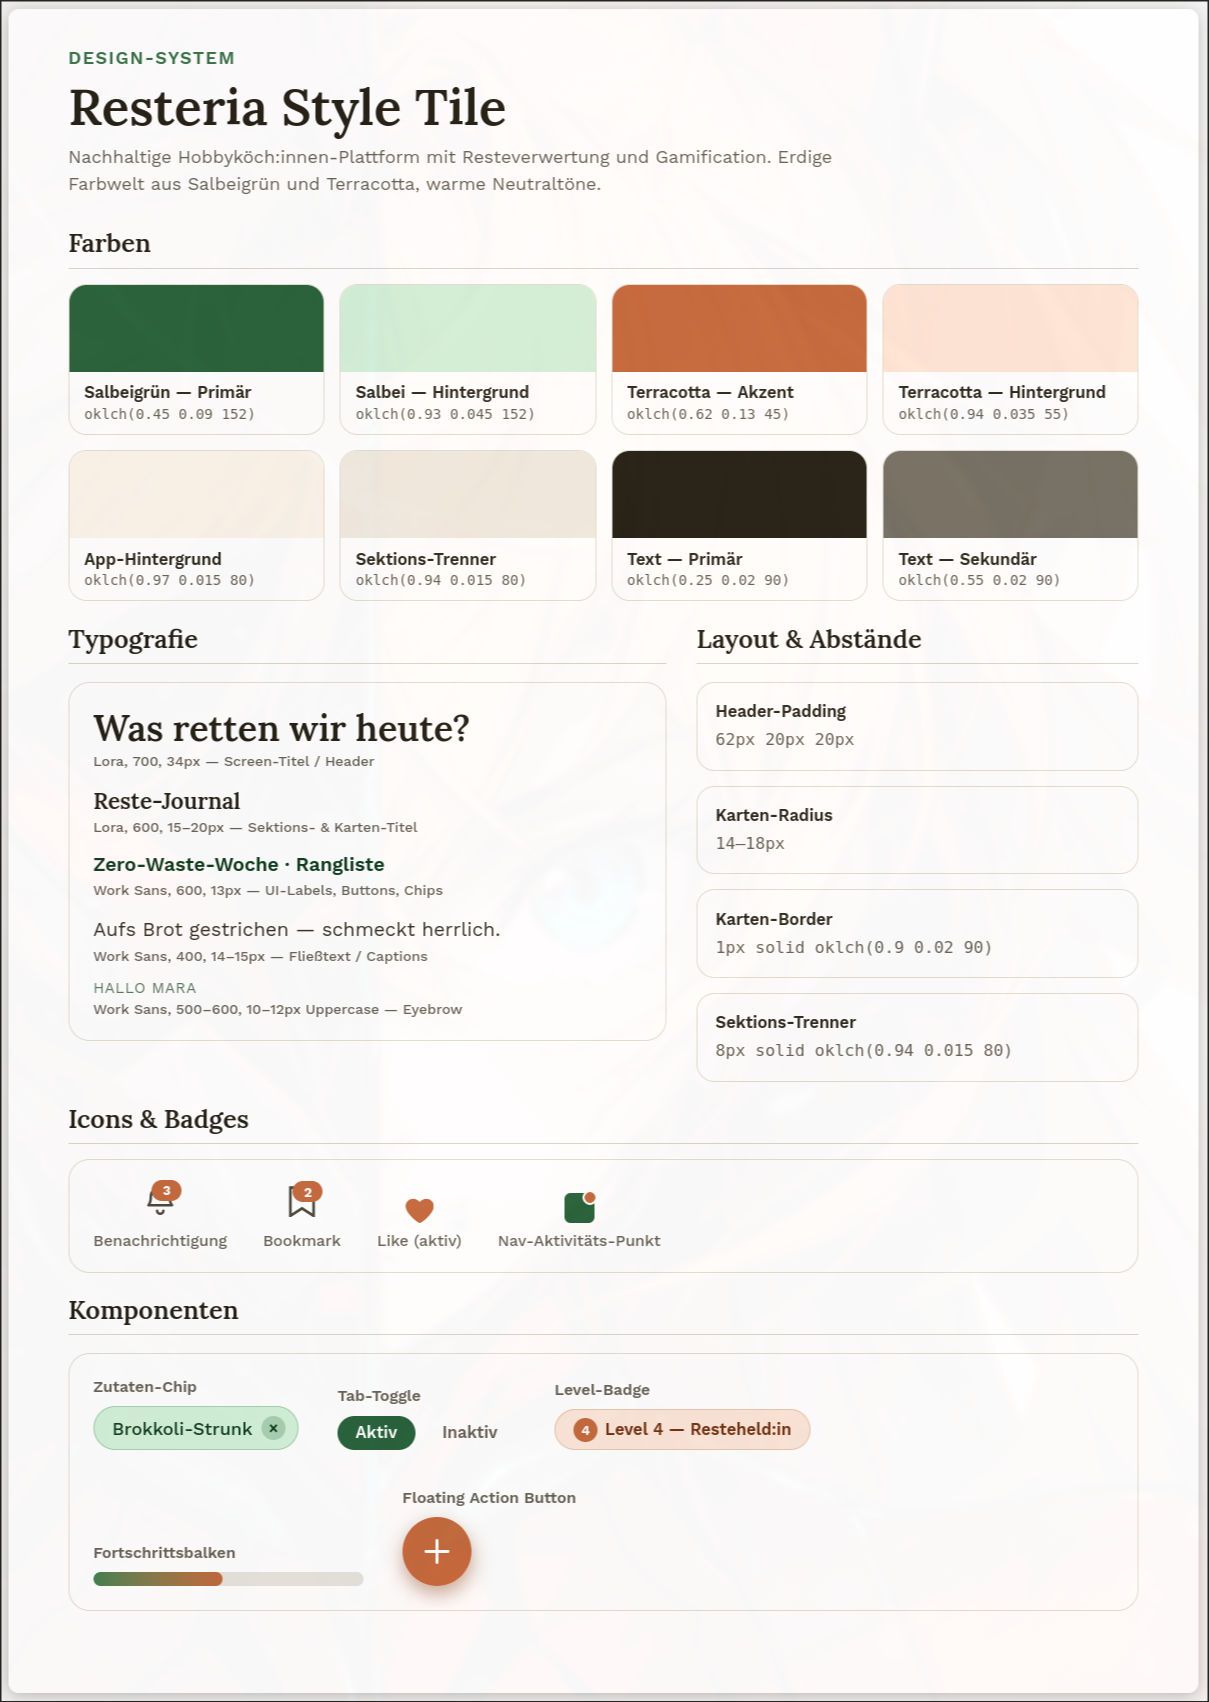
\includegraphics[height=0.85\textheight, keepaspectratio]{images/durchfuehrung/resteria_styletile.png}
\quelle{Erstellt mit dem Prompt \enquote{Erstelle einen Style Tile für das Projekt auf einer neuen Seite. Formatiere ihn als kompakter One-Pager im A4 Seitenformat} durch Anthropic, 2026 (Claude Design, Modell Claude Sonnet 5).}
\end{figure}

\section*{Anhang~C: UI/UX-Mockups Resteria}\label{sec:anhang_c}

\begin{figure}[H]
\caption{UI/UX-Mockup Resteria: Startseite mit Reste-Eingabe und Rezeptvorschlag}\label{fig:mockup_start}
\centering
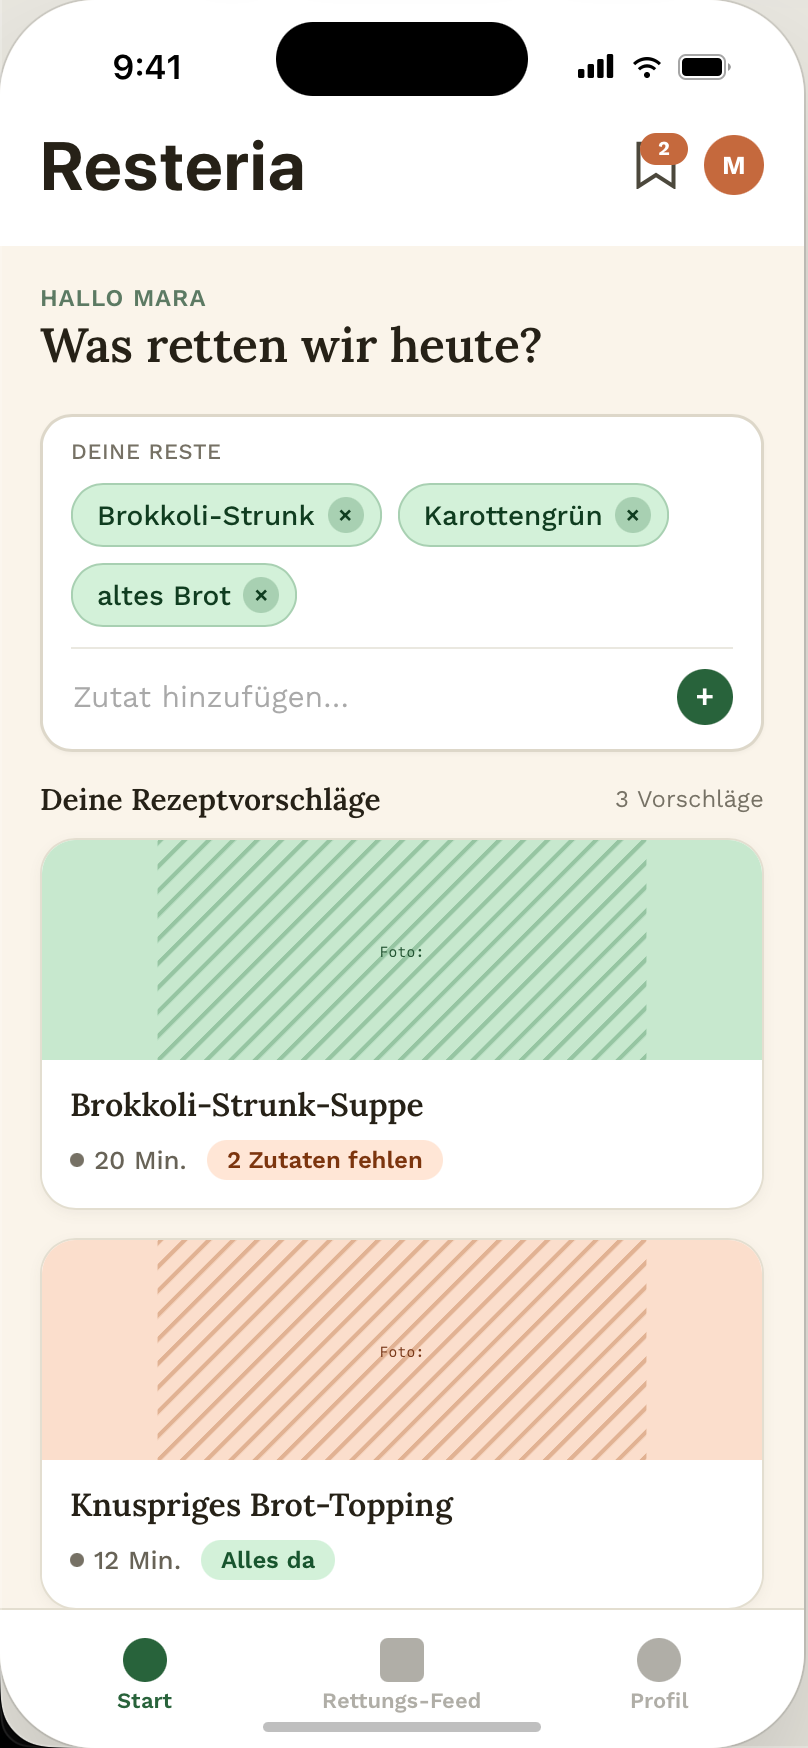
\includegraphics[height=0.55\textheight, keepaspectratio]{images/durchfuehrung/resteria_startseite.png}
\quelle{Erstellt mit dem Prompt \enquote{Mobiler App-Screen für Resteria, eine Social-Media-Plattform für nachhaltigkeitsorientierte Hobbyköche: Startseite mit Reste-Eingabefeld (Zutaten als Chip-Tags, z.\,B. Brokkoli-Strunk, Karottengrün, altes Brot) darunter Rezeptvorschläge als Karten mit Zubereitungszeit und fehlenden Zutaten. Verwende einen warmen, erdigen Look in Grün- und Terracotta-Tönen, keine Stock-Photo-Ästhetik}, in weiteren Iterationsschritten verfeinert, durch Anthropic, 2026 (Claude Design, Modell Claude Sonnet 5). Abbildung nachträglich manuell bearbeitet.}
\end{figure}

\begin{figure}[H]
\caption{UI/UX-Mockup Resteria: Startseite mit ausgeklappten gespeicherten Rezepten}\label{fig:mockup_start_bookmarks}
\centering
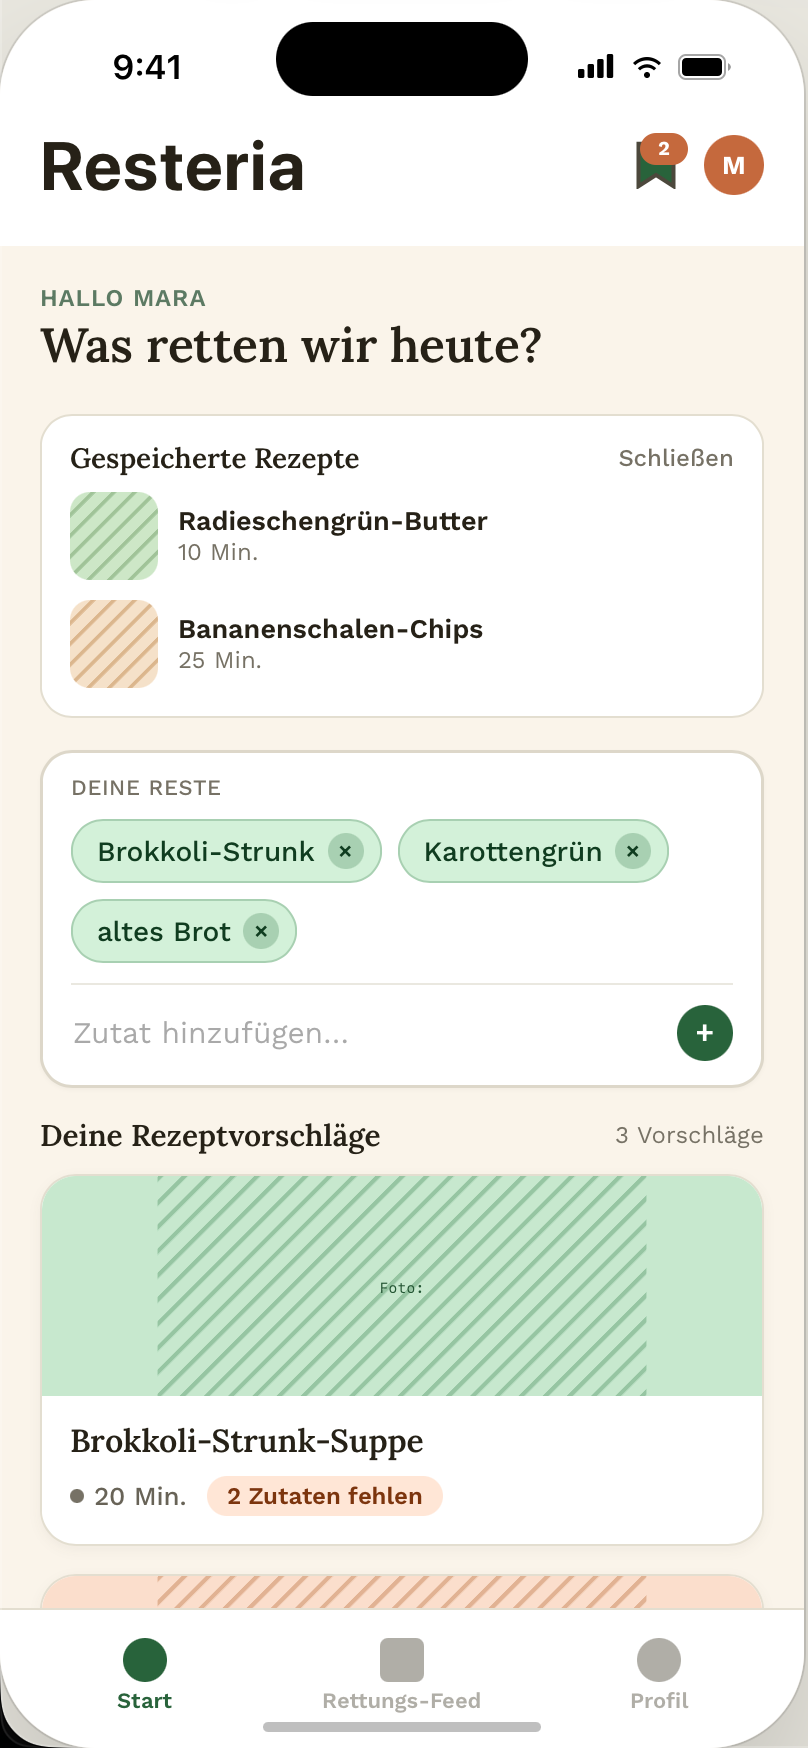
\includegraphics[height=0.55\textheight, keepaspectratio]{images/durchfuehrung/resteria_startseite_bookmarks.png}
\quelle{Erstellt mit dem Prompt \enquote{Ergänze ein über das Lesezeichen-Icon ausgeklappten Bereich \enquote{Gespeicherte Rezepte}, der zuvor per Lesezeichen markierte Rezeptvorschläge auflistet.}, in weiteren Iterationsschritten verfeinert, durch Anthropic, 2026 (Claude Design, Modell Claude Sonnet 5). Abbildung nachträglich manuell bearbeitet.}
\end{figure}

\begin{figure}[H]
\caption{UI/UX-Mockup Resteria: Rettungs-Feed}\label{fig:mockup_feed}
\centering
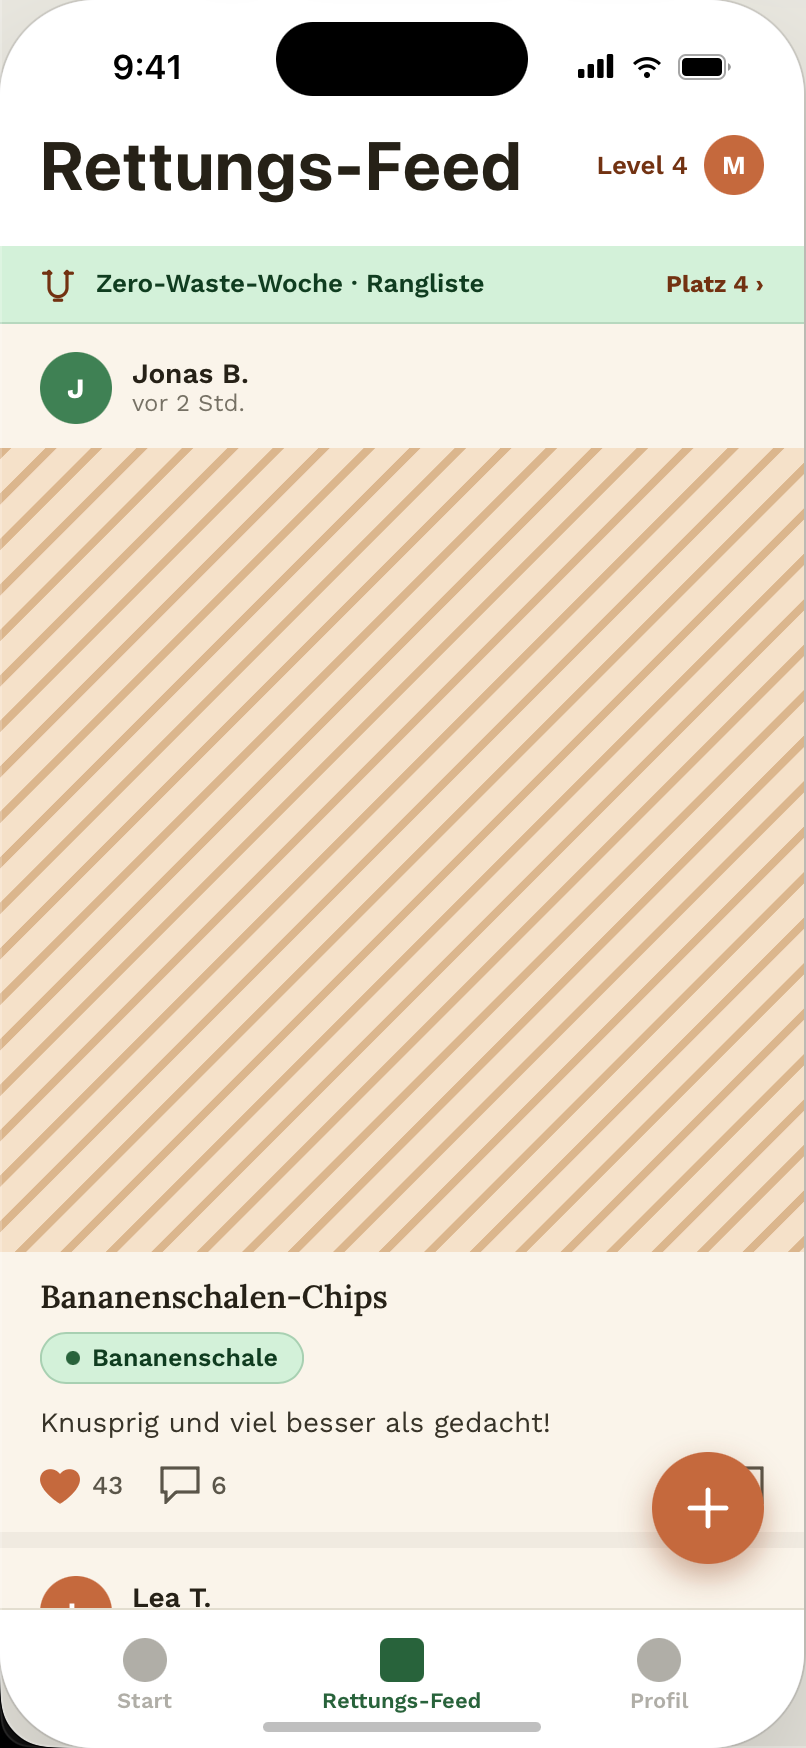
\includegraphics[height=0.55\textheight, keepaspectratio]{images/durchfuehrung/resteria_rettungsfeed.png}
\quelle{Erstellt mit dem Prompt \enquote{Rettungs-Feed im Social-Media-Stil mit Beiträgen, mit je ein Foto, Nutzernamen, Tags mit geretteten Zutaten sowie Like- und Kommentar-Icons. Warmer, erdiger Look in Grün- und Terracotta-Tönen, keine Stock-Photo-Ästhetik}, ergänzt um die Folge-Prompts \enquote{Ergänze am Rettungs-Feed-Screen einen schwebenden Terracotta-Plus-Button unten rechts zum Beitrag-Erstellen sowie ein schmales Challenge-Banner oben für die \enquote{Zero-Waste-Woche}-Rangliste}, in weiteren Iterationsschritten verfeinert, durch Anthropic, 2026 (Claude Design, Modell Claude Sonnet 5). Abbildung nachträglich manuell bearbeitet.}
\end{figure}

\begin{figure}[H]
\caption{UI/UX-Mockup Resteria: Profil mit Rettungspunkten und Reste-Level}\label{fig:mockup_profil}
\centering
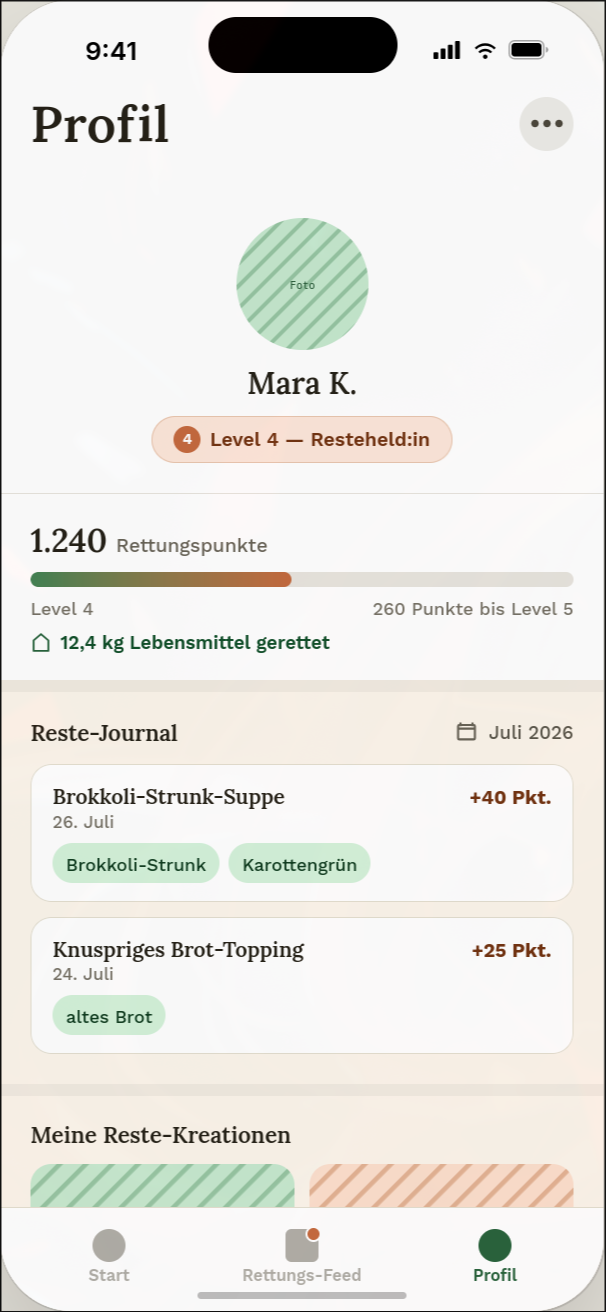
\includegraphics[height=0.55\textheight, keepaspectratio]{images/durchfuehrung/resteria_profil.png}
\quelle{Erstellt mit dem Prompt \enquote{Profilbereich mit Profilbild Platzhalter, Name und Reste-Level-Badge (z.\,B. \enquote{Level 4 - Resteheld}), Rettungspunkte-Fortschrittsbalken und einem Raster eigener geposteter Reste-Kreationen. Warmer, erdiger Look in Grün- und Terracotta-Tönen, keine Stock-Photo-Ästhetik}, ergänzt um die Folge-Prompts \enquote{Ergänze unterhalb des Rettungspunkte-Fortschrittsbalkens eine zweite, kleinere Kennzahl mit einer konkreten Mengenangabe, z.\,B. \enquote{12,4 kg Lebensmittel gerettet}}, in weiteren Iterationsschritten verfeinert, durch Anthropic, 2026 (Claude Design, Modell Claude Sonnet 5). Abbildung nachträglich manuell bearbeitet.}
\end{figure}


\end{document}
